% !TeX root = ba.tex

\section{Experiments}
\label{sec:experiments}

\subsection{Datasets and Network Architectures}

We trained models on each of the following benchmark data sets:

\begin{itemize}
	\item MNIST: $28\times28$ grayscale images of handwritten digits (60,000  images for training / 10,000  images for testing) \cite{mnist}
	\item Fashion-MNIST:  $28\times28$ grayscale images of fashion items (60,000 images for training / images 10,000 for testing) \cite{fashion}
	\item SVHN: $32\times32$ color images of house numbers (73,257  images for training / 26,032 images for testing) \cite{svhn}
	\item CIFAR-10: $32\times32$ color images (50.000  images for training / 10.000  images for testing) \cite{cifar}
\end{itemize}

Each of the four data sets consist of ten classes.

As baseline architectures we trained convolutional networks utilizing max-pooling,
batch normalization \citep{batchnorm} and dropout \citep{dropout}.
Training capsule networks can be comparatively more difficult in practice, therefore we had to carefully construct well-suited architectures:

For the MNIST data set we used three layer CapsNet like that of \citet{capsules}, but with only 64 convolutional kernels in the first layer. \\
For the Fashion-MNIST and the SVHN data sets we used CapsNets with two convolutional layers in the beginning, followed by the primary capsule layer and the class capsules. \\
Simple CapsNets however don't perform very well on more complex data like CIFAR-10 \citep{complex}, therefore we use a modified DCNet \citep{dcnet} with three convolutional capsule layers and a non-of-the-above category for the dynamic routing. \\
We train all CapsNets using margin loss and the reconstruction loss for regularization \citep{capsules}, and we use three iterations in the dynamic routing. \\
All CapsNets as well as ConvNets are trained with the Adam optimizer \citep{adam}. \\
For more details on the model architectures, please refer to the tables in ~\ref{lab:networks}.

The test accuracies of our networks on the respective data sets are displayed in Table~\ref{tab:accuracies}.
While these accuracies do not reach the state of the art, the similarity between the performances of the CapsNets and ConvNets indicates their suitability to the task of comparing adversarial robustness.

\begin{table}
	
	%\vskip 0.15in
	\centering%\scalebox{0.85}{
	\begin{tabular}{lcccc}
		\toprule
		Network       & MNIST & Fashion-MNIST & SVHN & CIFAR-10  \\
		\midrule
		ConvNet           & $99.39\%$ & $92.90\%$ & $92.57\%$ & $88.22\%$ \\
		CapsNet           & $99.40\%$ & $92.65\%$ & $92.35\%$ & $88.21\%$ \\
		\bottomrule\\
	\end{tabular}%}
	\caption{Test accuracies achieved by our networks.}
	\label{tab:accuracies}
\end{table}

For each of the data sets we compute adversarial examples using our four chose attacks in the following manner: \\
\todo{Make this less horrible}
We randomly select $1000$ each from the test set and attack them with DeepFool and the boundary attack.
For Carlini-Wagner (with hyperparameter $\kappa=1$) we calculate $500$ adversarial examples for randomly chosen images from the test set and randomly chosen target labels (but that are different from the true labels). In the case of the universal perturbation we divide the test set into ten parts and compute on each part ten adversarial perturbations.

We do not restrict the maximal perturbation norm for any of the attacks and hence the Carlini-Wagner, the boundary and the DeepFool attack only generate valid adversarial examples.
Regarding the universal perturbations, we terminate the algorithm once accuracy falls below $50\%$.
We found, that the universal perturbations generalize well: while only a tenth of the test set is used to generate each universal perturbation, they can reduce the test accuracy of the whole test set to $50\pm2.5\%$.

In Figure~\ref{tab:images} some examples of the product of the attacks on CIFAR-10 can be seen. The Carlini-Wagner, the boundary and the DeepFool attack result in humanly imperceptible adversarial examples. Only the universal perturbations are clearly visible. Furthermore we can observe some differences in the structure of the adversarial perturbations. While the black-box attack (boundary attacks) produces perturbations that resemble random noise, some noticeable patterns emerge in the perturbations of the white-box attacks. For more examples of adversarial images for this and the other data sets, see ~\ref{lab:images}.

\begin{center}
\begin{longtable}{rccc}
	
	CW & 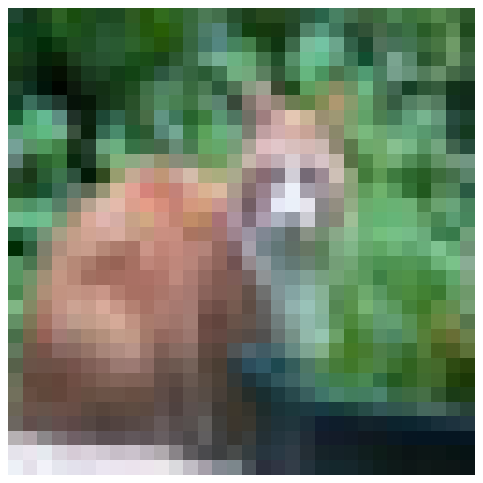
\includegraphics[height=2cm]{cifar10_carlini_wagner_orig.pdf} & 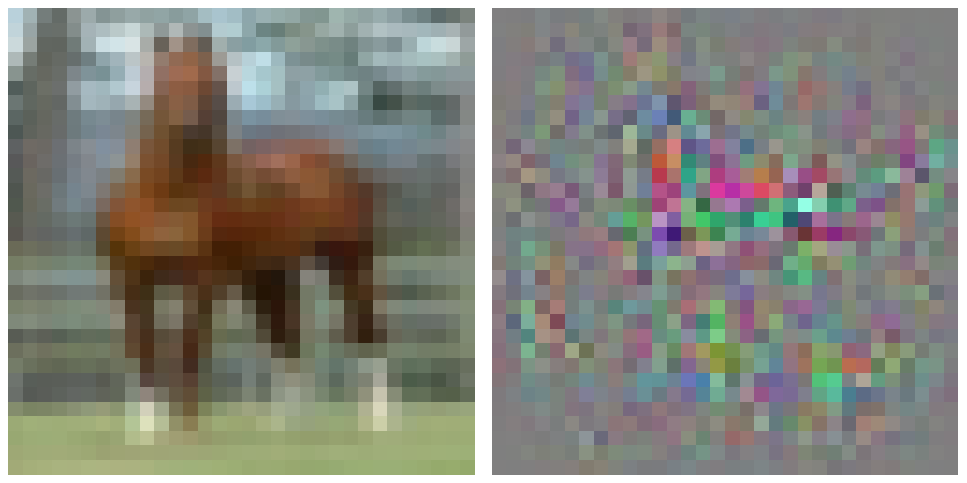
\includegraphics[height=2cm]{cifar10_carlini_wagner_caps.pdf} & 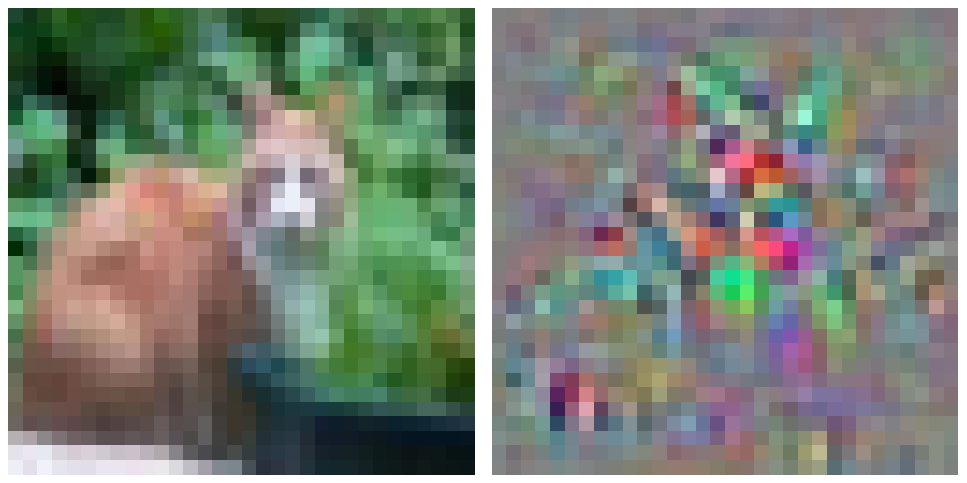
\includegraphics[height=2cm]{cifar10_carlini_wagner_conv.pdf}\\
	\\
	Boundary & 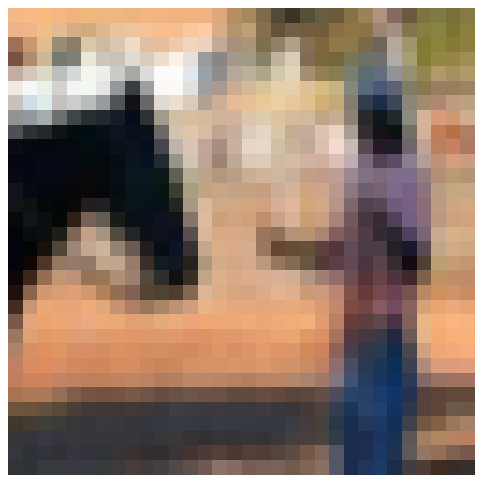
\includegraphics[height=2cm]{cifar10_boundary_attack_orig.pdf} & 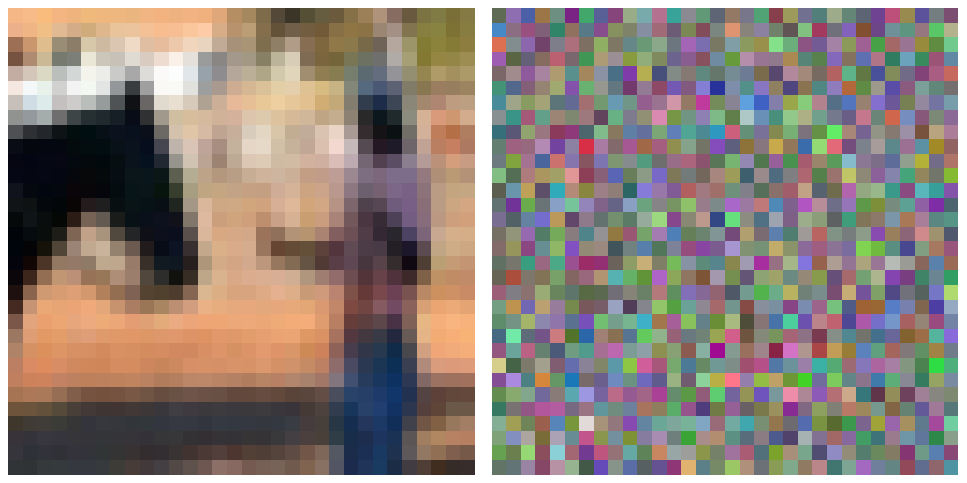
\includegraphics[height=2cm]{cifar10_boundary_attack_caps.pdf} & 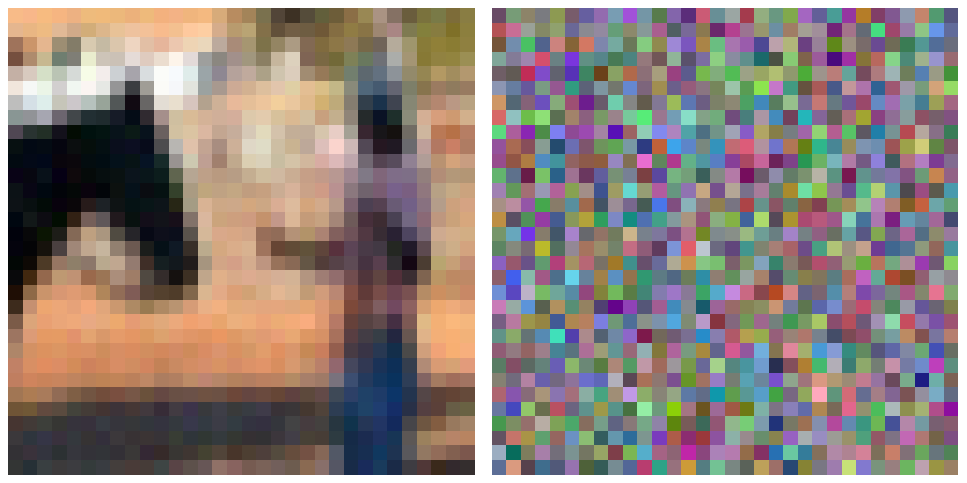
\includegraphics[height=2cm]{cifar10_boundary_attack_conv.pdf}\\
	\\
	DeepFool & 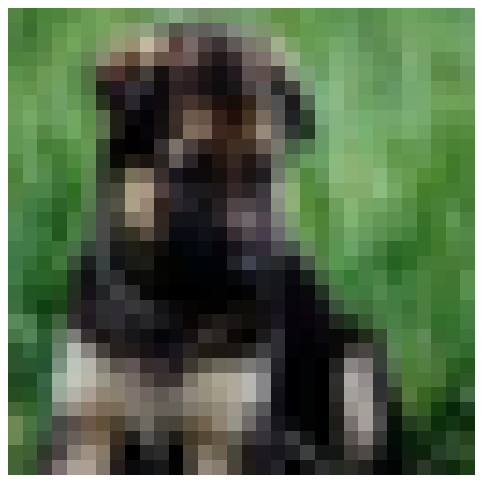
\includegraphics[height=2cm]{cifar10_deepfool_orig.pdf} & 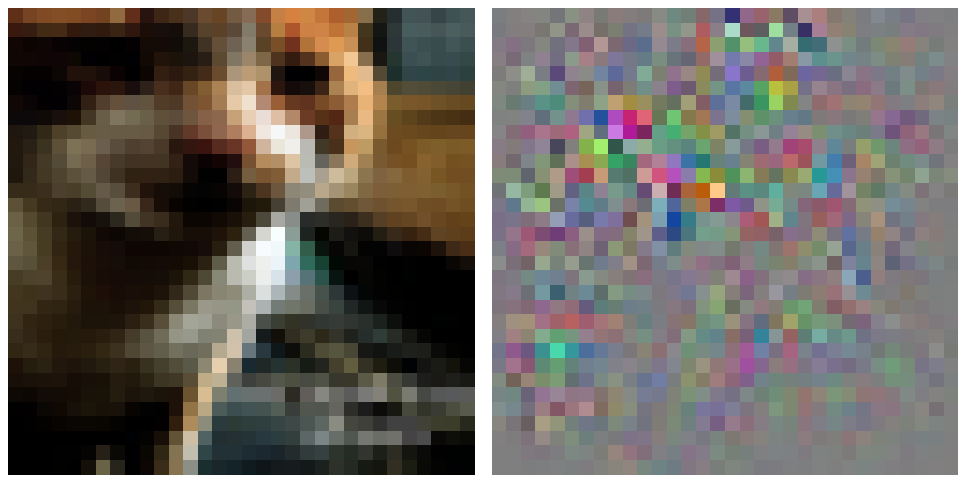
\includegraphics[height=2cm]{cifar10_deepfool_caps.pdf} & 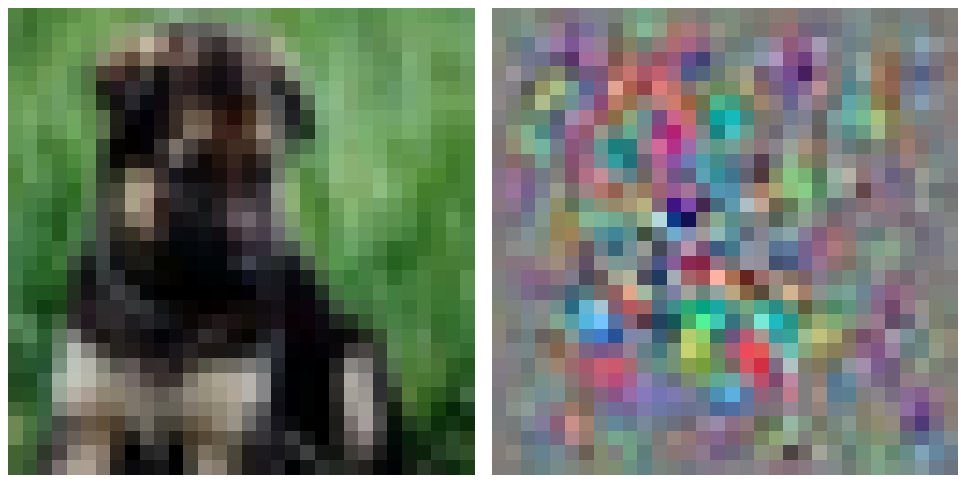
\includegraphics[height=2cm]{cifar10_deepfool_conv.pdf}\\
	\\
	Universal & 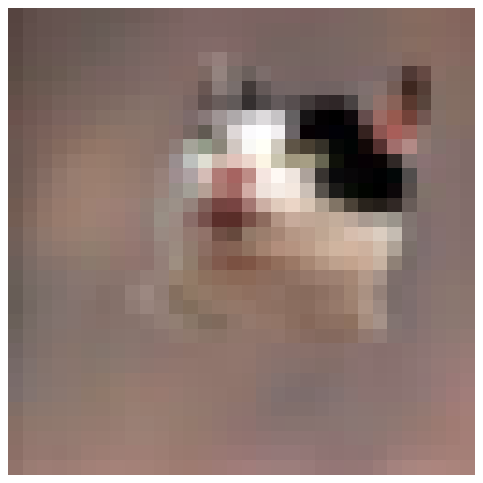
\includegraphics[height=2cm]{cifar10_universal_perturbation_orig.pdf} & 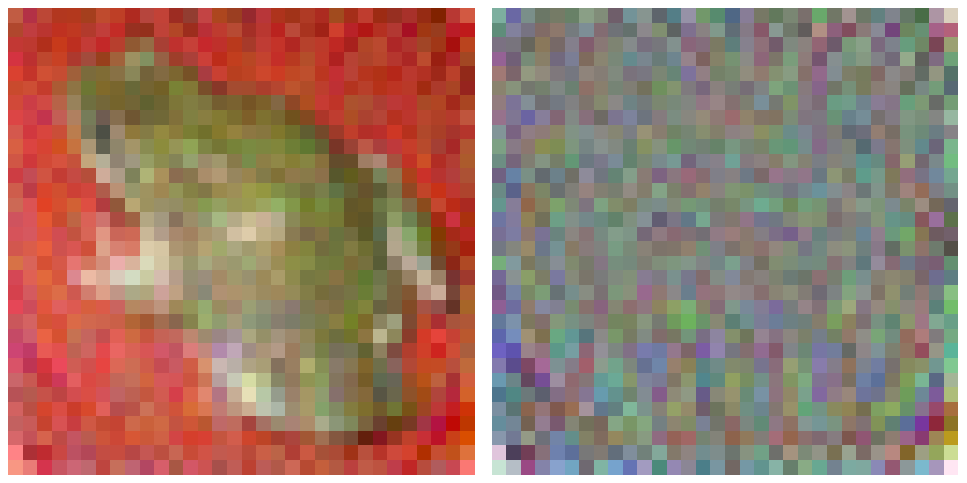
\includegraphics[height=2cm]{cifar10_universal_perturbation_caps.pdf} & 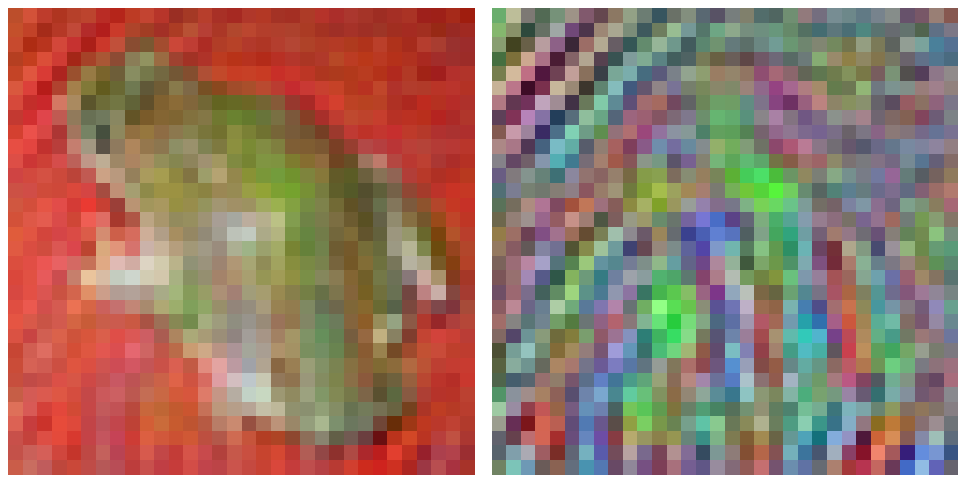
\includegraphics[height=2cm]{cifar10_universal_perturbation_conv.pdf}\\
	\\
\end{longtable}
	\captionof{figure}[Adversarial Examples on CIFAR-10]{Original images from the CIFAR-10 dataset (left), adversarial examples and perturbations for CapsNet (middle) and adversarial examples and perturbations for ConvNet (right). Pixel values of perturbation images are scaled for visibility.}
\label{tab:images}
\end{center}



\subsection{Robustness to Adversarial Attacks}

\begin{table}
	\centering\
	\begin{tabular}{llcccc}
		\toprule
		Attack & Network       & MNIST & Fashion & SVHN & CIFAR-10  \\
		\midrule
		\multirow{2}{*}{CW} & ConvNet & {$1.40$} & $0.51$ & $0.67$ & $0.37$ \\
		& CapsNet            & $1.82$ & {$0.50$} & {$0.60$} & {$0.23$} \\
		\midrule
		\multirow{2}{*}{Boundary} & ConvNet & {$3.07$} & $1.24$ & $2.42$ & $1.38$ \\
		& CapsNet            & $3.26$ & {$0.93$} & {$1.88$} & {$0.72$} \\
		\midrule
		\multirow{2}{*}{DeepFool} & ConvNet & {$1.07$} & {$0.31$} & {$0.41$} & $0.23$ \\
		& CapsNet           & $2.02$ & $0.55$ & $0.80$ & {$0.16$} \\
		\midrule
		\multirow{2}{*}{Universal} & ConvNet & {$6.71$} & {$2.61$} & {$2.46$} & {$2.45$} \\
		& CapsNet           & $11.45$ & $5.31$ & $8.59$ & $2.70$ \\
		\bottomrule\\
	\end{tabular}
	\caption[Average Perturbation Norms]{Average perturbation norms for each attack and architecture.}
	\label{tab:norms}
\end{table}
		
\begin{table}
	\centering
	\begin{tabular}{llcccc}
		\toprule
		Attack & Network       & MNIST & Fashion & SVHN & CIFAR-10  \\
		\midrule
		\multirow{2}{*}{CW} & ConvNet & $0.8\%$ & $1.2\%$ & $2.8\%$ & $2.4\%$ \\
		& CapsNet            & $2.0\%$ & $2.0\%$ & $3.8\%$ & $2.0\%$ \\
		\midrule
		\multirow{2}{*}{Boundary} & ConvNet & $8.8\%$ & $9.5\%$ & $10.5\%$ & $13.4\%$ \\
		& CapsNet            & $14.2\%$ & $14.6\%$ & $12.9\%$ & $26.1\%$ \\
		\midrule
		\multirow{2}{*}{DeepFool} & ConvNet & $4.3\%$ & $8.5\%$ & $13.5\%$ & $11.8\%$ \\
		& CapsNet           & $0.9\%$ & $10.9\%$ & $10.8\%$ & $14.1\%$ \\
		\midrule
		\multirow{2}{*}{Universal} & ConvNet & $4.9\%$ & $20.4\%$ & $35.0\%$ & $25.9\%$ \\
		& CapsNet           & $38.2\%$ & $25.7\%$ & $53.4\%$ & $47.2\%$ \\
		\bottomrule\\
	\end{tabular}
	\caption[Transfer Fooling Rates]{Fooling rates of adversarial examples calculated for a CapsNet and evaluated on a ConvNet and vice versa. For the universal attack we report the accuracy on the whole test set.}
	\label{tab:transfer}
\end{table}

\subsection{Structural Analysis of Adversarial Examples}

While we have found, that CapsNets are not necessarily more robust against adversarial attack, the low success rate of the transfer attacks suggest, that there may be some structural difference between adversarial examples computed for ConvNets and those computed for CapsNets.

\subsubsection{Universal Attack t-SNE}

We used t-SNE \citep{tsne} to make a scatter plot.
\begin{figure}
	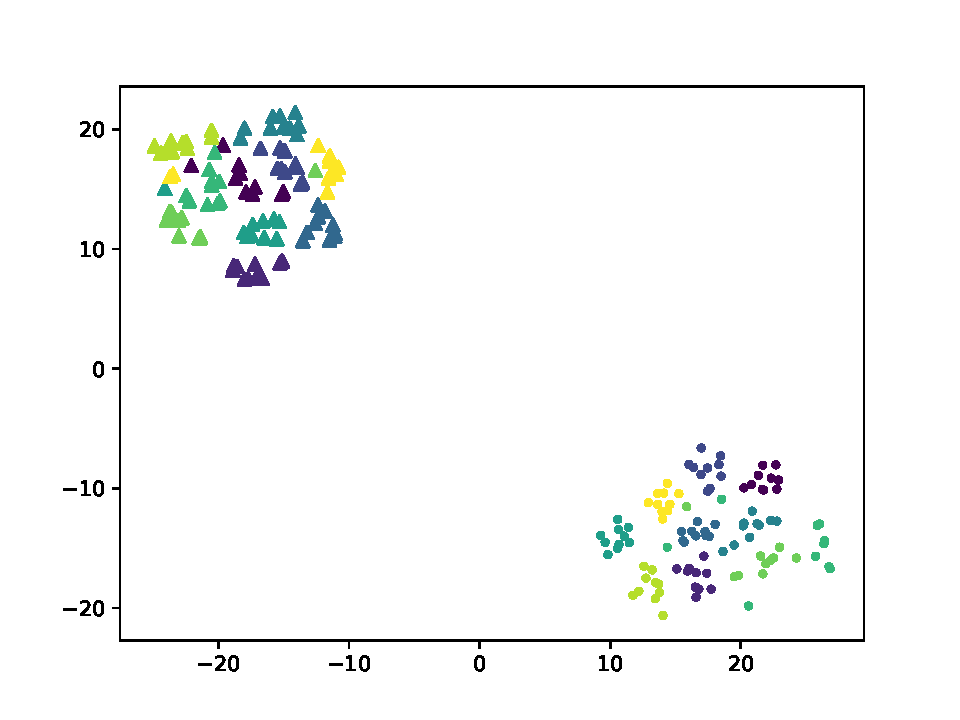
\includegraphics{tsne.pdf}
	\label{fig:tsne}
	\caption[t-SNE Plot of Universal Perturbations]{Two dimensional embedding of the universal perturbations on CIFAR-10 calculated using t-SNE \citep{tsne}. The upper right cluster represents perturbations computed on a ConvNet, whereas the cluster in the lower left represents those calculated on a CapsNet. Perturbations with the same color were created using the same subset of test data.}
\end{figure}




\subsubsection{SVD}
\citet{universal} considered singular values of the matrix containing normalized adversarial examples to determine, if adversarial examples lie in a low dimensional subspace. \\
For this purpose, let us denote with $\delta(x)$ the minimal adversarial perturbation for the input $x \in [0,1]^n$,
and $ N = \begin{bmatrix}
\frac{\delta(x_1)} {\norm{\delta(x_1)}},  ...,  \frac{\delta(x_k)} {\norm{\delta(x_k)}} 
\end{bmatrix}
\in \mathrm{R}^{n \times k}
$ for some $x_1, ..., x_k$ in the test set. \\
$\delta(x)$ is orthogonal to the decision boundary, assuming it is reasonably smooth, therefore the singular values of N give us information about the decision boundary. For example, for an binary linear classifier, N would have a rank of one, i.e. only one non-zero singular value.

In this regard we find little difference between CapsNets and ConvNets.

\begin{figure}
	\centering
	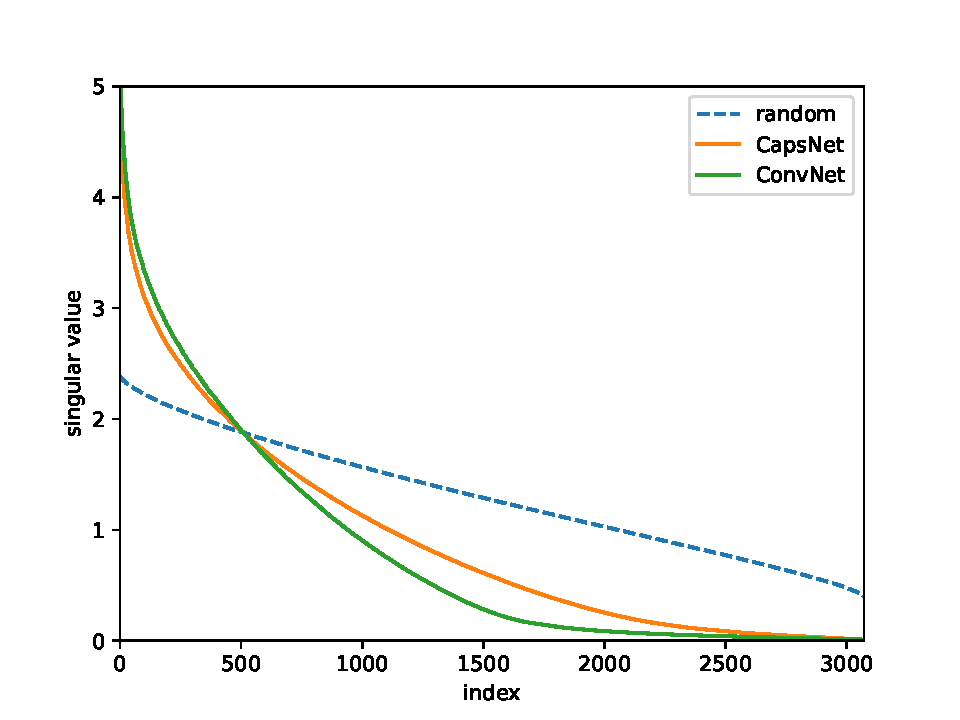
\includegraphics[width=.9\textwidth]{svd_cifar10.pdf}
	\caption{CIFAR-10}

	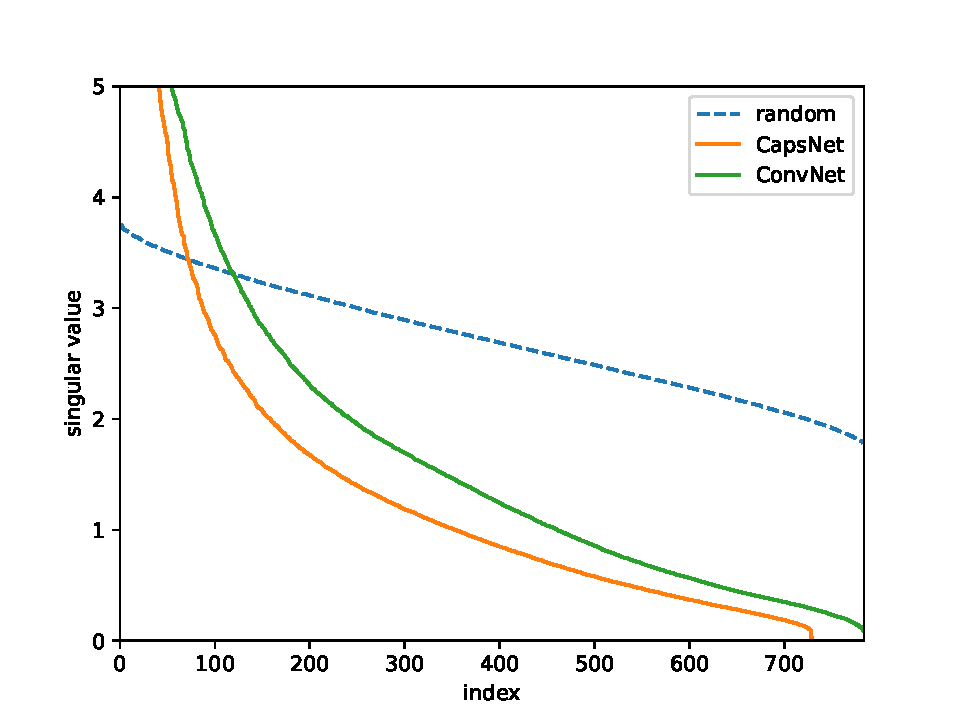
\includegraphics[width=.95\textwidth]{svd_mnist.pdf}
	\caption{MNIST}
	\caption{Singular Values of Matrix Containing Normal Vectors To the Decision Boundary}
	\label{fig:svd}
\end{figure}